\documentclass[a4paper,12pt]{scrartcl}

\usepackage{titlesec}

\usepackage[swedish,english]{babel}
\usepackage{url}
\usepackage{booktabs}
\usepackage[toc,page]{appendix}
\usepackage{multirow}
\usepackage{amsmath}

\usepackage{graphicx}

\title{Wikipedia Information}
\author{Linus Hansson, Amelia Andersson, Per Classon\\Anton Warnhag, Johan Ekstr\"{o}m} % � = \"{0}

\begin{document}

\maketitle
\selectlanguage{english}


\begin{abstract}
This article discusses several methods to automatically summarize texts. We implemented a keyphrase extraction method in order to find relevant information from Swedish Wikipedia articles based on keywords. We found that the implementation could return relevant summaries, especially if only the first few tf-idf-ranked documents were used for keyphrase extraction.
\end{abstract}

\section{Introduction}
\subsection{Background}
Today, information is becoming abundant. There is a vast amount of information available on the Internet and this amount is only growing in size. Because of the expanding set of relevant data, it is becoming more and more important to construct relevant overviews, which saves one from sifting through a complete corpus in order to get a general idea of a topic. Another problem may arise from the expansion of information itself; as it grows, previous summaries may become obsolete. Automatic information abstraction is therefore an important problem to solve.

Text summarization is a way of solving this problem in its textual form. The idea is that texts have inherent structures that can be exploited in order to find relevant data. Different methods such as abstraction (which attempts to summarize the text in natural language) and extraction (which returns important sentences from the text itself) may be employed, either by themselves or in conjunction.

\subsection{Purpose}

The purpose of this project was to build a tool that would automatically return context information of any given query. This was to be done using a text summarization method with information specifically collected from Wikipedia articles. This paper aims to add a theoretical background to this endeavor, as well as to give a detailed report on how the tool was implemented and evaluated. 

\section{Previous/Related work}
There are many different algorithms one can use to summarize a text. Before finally deciding on using Continuous LexRank (see Chapter \ref{sec:lexrank}) we spent quite a lot of time looking into some of the alternative algorithms. The results of our study are presented in the following subchapters.

\subsection{Introduction: Extractive vs. Abstractive }
In the field of natural language processing, one differs between extractive and abstractive text summarization. 

Extractive summarization produces a summary of a text cluster by choosing a subset of the sentences in the cluster. The way to choose sentences may differ between methods, but each method should have some way of giving each sentence a score to be able to sort them according to relevance.  

Abstractive text summarization on the other hand involves paraphrasing sections of the cluster. By definition it involves generating text not necessarily appearing in the original documents. This generation involves abstracting words used to broaden themes and synonyms of the words in the texts. This part of the field of summarization is much less developed than extractive methods, mostly because it involves another field still in its early stages: that of natural language generation. NLG is the process of turning knowledge based information into natural language that is more easily understandable to humans.

The following subsections give examples of different text summarization methods and how they are used. The two first examples, Lexical Chains and LexRank, are extractive methods, while the last example, Opinosis, is an abstractive method. 


\subsection{Lexical Chains}
Capturing the key points of a text is essential in automatic text summarization. A rather sophisticated approach to this is to use Lexical Chains. A lexical chain can be thought of as a list of words, most commonly nouns, absorbed from a document. These are meant to form a representation of the key themes of the text.

Lexical Chains exploit lexical cohesion between sentences. Lexical cohesion involves the selection of a lexical item that is in some way related to one occurring previously. Repetition, i.e several occurrences of identical words is one form of lexical cohesion, but cohesion also includes synonyms, near synonyms or hierarchical connections. When cohesive elements occur over a number of sentences a cohesive chain is formed.

Implementing a Lexical Chains algorithm requires a database of words and their connections to other words. A resource that is commonly used to this end is WordNet. WordNet lists all the related words to any given word together with the relation. Given that only nouns are treated a Part-of-Speech tagger is also needed to single out the nouns of the text. These nouns are then grouped into chains according to the cohesive relations mentioned above. In the end the resulting chains are ranked according to strength. Strength can be determined using a scoring system depending on the length of the chain and the relationships it holds. These will then reveal the central themes of the text and a summary can be formulated. \cite{LexicalChains} \cite{LexChains}


\subsection{LexRank} 

\subsubsection{Degree Centrality}
Degree Centrality makes the assumption that many sentences in a cluster of related documents are somewhat similar to each other. The way in which Degree Centrality uses this assumption is by viewing the text cluster as an undirected graph. Firstly, words are given a tf-idf score and the similarity between each pair of sentences, $(x,y)$, are calculated using a idf-modified-cosine score.

\begin{equation}
idf\text{-}modified\text{-}cosine(x,y) = \frac	{\sum_{w \in x,y}{tf_{w,x} tf_{w,y} (idf_w)^2}} {\sqrt{\sum_{x_i \in x} {(tf_{x_i,x} idf_{x_i})^2} } \cdot \sqrt{\sum_{y_i \in y} {(tf_{y_i,y} idf_{y_i})^2} }}
\end{equation}

where $tf_{w,s}$ is the number of occurrences of the word $w$ in the sentence $s$.
Each sentence in the cluster is then represented by a node. Two sentence nodes are only connected if their similarity score exceeds a certain threshold. With this graph representation, a simple way to assess the centrality of a sentence is to count the number of similar sentences, i.e the number of neighbors the node has. This algorithm sorts all sentences according to their centrality score, in descending order, and a summary can be chosen as the k highest ranking sentences. 

The Degree Centrality algorithm is interested in all similar pairs of sentences, and does not take into account the actual value of the similarity as long as they are above a certain threshold. In the graph view described above, it only counts the number of sentences that are similar according to the threshold and thus in effect removing the edges with lower similarity scores. The choice of the threshold can greatly influence the result - a high threshold will eliminate almost all similarities and a low threshold might take the unwanted weak similarities into account as well. \cite{LexRank}


\subsubsection{LexRank}
LexRank is an extension of Degree Centrality. The idea behind LexRank is that all edges are weighted and therefore more or less important. In Degree Centrality, if several irrelevant sentences are similar to each other, those sentences will have a high centrality score due to the fact that they are neighbors in the centrality graph. The LexRank extension tries to eliminate this unwanted behaviour.

The way LexRank does this is to use the centrality of the neighboring sentences. Each sentence has a specific centrality value, $p$, and shares an equal portion of this value to all its neighbors. This can be formulated as the following equation:

\begin{equation} \label{equ:lex}
p(u) = \sum_{v \in adj(u)}{\frac{p(v)}{deg(v)}}
\end{equation}

where $p(s)$ is the centrality of sentence $s$, $deg(s)$ is the number of neighbors of $s$ and $adj(s)$ is the set of neighbors of $s$.
This equation is however unsolvable, but Erkan and Radev suggests a solution to this equation using the PageRank algorithm (hence the name LexRank, Lexical PageRank) together with some form of iterative method in order for Equation \ref{equ:lex} to converge, for example Power Iteration. 


\begin{equation}
p(u) = \frac{d}{N}+(1-d) \cdot \sum_{v \in adj(u)}{\frac{p(v)}{deg(v)}}
\end{equation}

where $d$ is the possibility to perform a random jump between the sentences and $N$ is the total number of sentences.
\cite{LexRank}

\subsubsection{Continuous LexRank} \label{sec:lexrank}
Neither Degree Centrality nor LexRank take the similarity weight between sentences into consideration, only how many similar sentences there are. The difference between LexRank and Continuous LexRank is that the cosine score is used directly in the PageRank algorithm. The graph will be denser but weighted.

\begin{equation}
p(u) = \frac{d}{N}+(1-d) \cdot \sum_{v \in adj(u)}{\frac{idf\text{-}modified\text{-}cosine(u,v)}{\sum_{z \in adj(v)}{idf\text{-}modified\text{-}cosine(z,v)}}}p(v)
\end{equation}

These two variants of LexRank may also differ in the aspect of what counts as similar sentences. In Continuous LexRank the threshold mentioned earlier is removed, and all values of similarity are accepted. \cite{LexRank}


\subsection{Opinosis}
Opinosis is a concept intended to condense what the authors call �highly redundant opinions�. Specifically this means that it is designed to summarize comments on products of different kinds, such as you might find in below a product page in an online store or beneath a review of a movie. The idea is that the method creates a summary that includes the most repeated parts.

It does this by generating a graph of the words used, where every node stands for some specific word and points to all the other word-nodes that its word closely precedes (within a few words) in the chosen collection of text, along with how many times it comes up preceding that word. So this graph tells you which strings of words come up most frequently in the collection. Given some lower limit for how many times a string needs to show up to be considered, those that do are then used to construct a summary using some rather simple concepts from natural language generation, NLG, concerning the structure of sentences. In effect, the algorithm creates a rough intersect of the collection�s sentences, leaving out the parts that only show up in individual or few sentences.

Opinosis is not truly abstract (the authors calls it shallowly abstract) because it does not generate words that are not in the subject collection. But it does create sentences that were not in that collection, and sidesteps many of the difficulties with NLG by utilizing its sentence structure. \cite{opiniosis}


\section{Method}
Our idea at first was to combine the concept of a word graph, as used in Opinosis, with the generation of the most important sentences from an extractive method such as LexRank. But because LexRank does not generate the highly redundant collection of sentences needed by Opinosis, we would modify LexRank from doing an intersection to instead doing the equivalent of a union. Using a word graph we would identify shared parts of the sentences, for example names, and �fuse� the parts that were not shared based on these.

However, such fusing turned out to be very difficult if we intended to return something that could compete in legibility and completeness of the summary compared with simply putting the most important sentences returned directly by LexRank in line after each other. It also proved outside the scope of how much time we could spend on this project, and due to this we ended up implementing Continuous LexRank on its own.

We also planned to build a small and simple GUI in which a user could define her search strings. A GUI was not specified in the project description, but we considered it an important addition to our program as it was meant for human use.


\subsection{Our program}
We coded the algorithm in Java and implemented it in such a way that we could change different parameters in-between runs (these parameters are described in Chapter \ref{sec:eval}, Evaluation). Even though this is not included in the Continues LexRank algorithm, we chose to have a limit for when sentences are to be considered similar, more specifically when two sentences should be neighbors in the graph view. This limit was chosen to be 0.1 (a value of 1.0 means that the sentences are identical and 0.0 means that they are the opposite). We noticed a small improvement in results when doing this. 

Due to Wikipedia's tendency to have a short summary of the subject at hand at the beginning of each article, we added a parameter with which we could control how early on in the text a sentence had to show up to be considered for the resulting summary. In addition to this, we also built a small GUI in which a user could define her search strings and view the results sent back from the program, i.e. the program's summarization of the search topic. 

Between our LexRank algorithm and our GUI, we implemented a processing layer. The task of this layer was to convert the search string from the user to an Apache Solr url and then to decode the result from Solr. When performing a search in an Apache Solr database, one can choose between a few output formats of the result. We chose to receive the output in the JSON format (Javascript Object Notation) and use the JSON-simple library to decode the result and gather the sentences from the Wikipedia articles. From the Wikipedia articles you can gather a lot of information about revisions and user edits, but we were only interested in the title and text of the current revision of the articles and therefore only extracted these.


\begin{figure}[htbp]
   \centering
   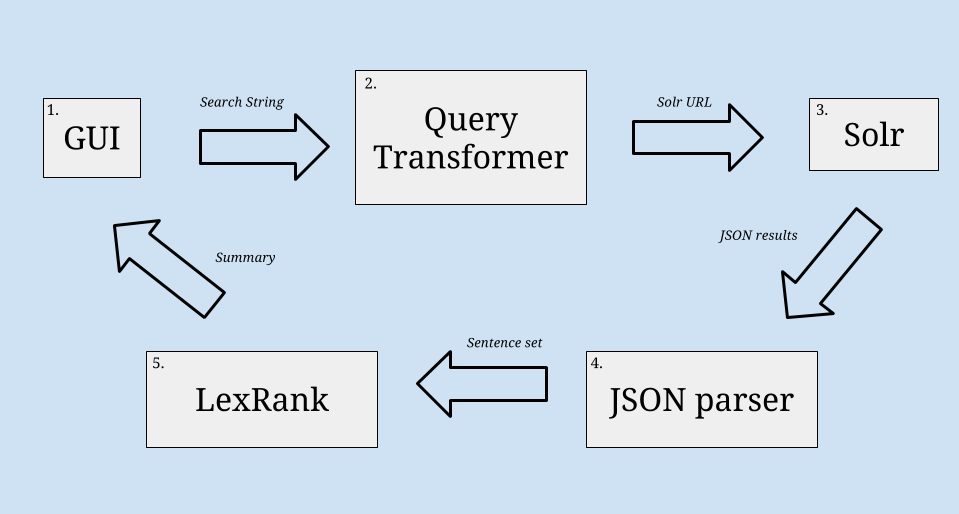
\includegraphics[scale=0.4]{IrProjectWorkFlowMedSiffror.png}    
   \caption{Our system as a workflow chart, with numbers demonstrating the order and the arrows showing the input/output to the different steps}
   \label{fig:workflow}
\end{figure}


All sentences continued to the LexRank implementation, which ranked the sentences according to relevance to the query. The highest ranked sentences from the LexRank algorithm were then sent to back to the GUI along with the titles of the Wikipedia article containing the sentence. 

\subsection{Resources}
The following subsections list the resources we used for our implementation.

\subsubsection{Wikipedia database} \label{sec:wiki}
Due to the massive size of the english-language edition of Wikipedia, we decided to use the much smaller swedish-language Wikipedia as our source of data. Wikipedia provides their data for download in the format of XML (Extensible Markup Language). By using the database Apache Solr, it was then possible to import the XML-data and save the articles in a searchable format. As Wikipedia contains a lot of unwanted articles, such as redirects, portals, templates and categories; a regular expression pattern was used to skip those documents.  \cite{wikidb}

\subsubsection{Apache Solr}
Solr is an open source search platform with features such as full-text search which is very scalable. It is implemented in Java and runs as a standalone server. It comes with a REST-api (Representational state transfer) where you can search by doing simple GET-requests. The results of these GET-requests were then parsed and used in our algorithm. \cite{solr}

When doing full-text searches, Solr uses, by default, a tf-idf scoring method with some modifications for ranking the articles. They have made what they call a Lucene's Practical Scoring Function, which it is based on the Vector Space Model (VSM) and uses the tf-idf scoring system. These scores can be combined with a document boost (which is predefined scores of documents that should be ranked higher) and a query boost (some words in queries can be given higher priority). \cite{lucene}

\subsubsection{JavaFX}
JavaFX is a GUI library for Java and a software platform for creating and delivering rich internet applications (RIAs). We used it to create a desktop application from which a Wikipedia search could be done. \cite{JavaFX}

\subsubsection{JSON-simple}
JSON-simple is a simple Java toolkit for encoding or decoding JSON text. We used it in order to decode the result from a Apache Solr query. \cite{JSONsimple}


\section{Evaluation}
\label{sec:eval}
\subsection{Design}
To measure the efficiency of our program and algorithms we constructed an experiment where we calculated the precision of a set of 16 predefined queries (see appendix \ref{app:queries}). For each query we evaluated the summary we got back and graded it using a three graded scale as shown in Table \ref{tab:desc} below.

\begin{table}[htbp]
   \centering
   \begin{tabular}{@{} cc @{}} 
      \toprule
      Grade & Description \\
      \midrule
      0 & Not relevant \\
      1 & Relevant information \\
      2 & Relevant description \\
      \bottomrule
   \end{tabular}
   \caption{The grades used to evaluate our queries.}
   \label{tab:desc}
\end{table}


The program had four different parameters that were changed during evaluation, and all queries were tested with each parameter setting. The parameters we used were:

\subsubsection*{1. Maximum number of documents returned from Solr.}
For the first parameter we tested the values one and five. With this parameter set to one, we only used the top ranked document from Solr in our summarization, and with the parameter set to five, we used the top five documents from Solr in the summarization. Unfortunately, we never managed to remove all of the unwanted articles mentioned in Chapter \ref{sec:wiki} and as a consequence of this, we had to use a guard in our implementation to skip documents of those types while summarizing.

\subsubsection*{2. Minimum number of sentences required in a document.}
For the second parameter we used the values one and ten. This parameter meant that we excluded all documents containing less than one or ten sentences. There is a substantial amount of Wikipedia articles that are either not complete, or whose only function is to refer to other articles. We did not want our summarization to be built on any of these articles.

\subsubsection*{3. Minimum number of words in a sentence.}
When parsing a Wikipedia article we could end up with very short �sentences�, namely words that were in fact a link, a header, or something else entirely. To see how much these �sentences� would affect the result we used the third parameter to skip some of them. The values we used were zero and five. With zero as the limit, we accepted all sentences, even the ones described here and with five as the limit, we skipped these sentences.

\subsubsection*{4. Maximum position of a sentence in a document.}
The last parameter told our program from where in the articles the summarization was to be extracted. We ran LexRank on the entire document, but when selecting the summary we wanted to be able to use the general layout of the Wikipedia article where there is usually somewhat of a summary of the article in the beginning. The values we tested were five, ten and one thousand. The value one thousand can be interpreted as the entire document since most articles contain less than one thousand sentences.


\subsection{Results}

The maximum score of each test is 32. A maximum score would correspond to the program delivering accurate summaries of each of our 16 test queries (see Appendix \ref{app:queries}) for the current test setting. The average score we obtained from running all different permutations of parameter values was 12.125, but depending on parameter settings we swayed between a score of 18 at the high end and 5.2 at the lower, suggesting there lies some importance in the choice of these. For the different parameters in our evaluation we calculated some average scores:

\begin{table}[htbp]
\centering
\begin{tabular}{|c|c c|}
\hline
Parameter & Value & Averaged Score \\
\hline
\multirow{2}{*}{Max no. docs} & 1 & 14.35 \\
& 5 & 9.9 \\
\hline
\multirow{2}{*}{Min. sentences for docs} & 1 & 13.78 \\
& 10 & 10.47 \\
\hline
\multirow{2}{*}{Min. words for sentence} & 0 & 11.78 \\
& 5 & 12.47 \\
\hline
\multirow{3}{*}{Max sentences position} & 5 & 12.47 \\
& 10 & 11.53 \\
& 1000 & 10.18 \\
\hline
\end{tabular}
\caption{Average scores from the evaluation where the parameter values were changed. Full data can be seen in appendix \ref{app:results}.}
\end{table}
These parameters work in combination, and changing one affects the others. Still, these averages should give some indication as to the relative importance of the different variable values.


\section{Discussion}

First, some notes on the different parameters we use:

\begin{itemize}
\item
It was interesting to see how much the first parameter (number of documents) influenced the result, from an average score of 9.9 when using five documents to 14.35 for using just the top ranked document. Without studying the similarities and disparities of the documents returned by Solr further, it is not possible to draw any more conclusions.

\item
We also tried to filter out very short documents/articles since we thought their scores would not reflect well on the actual importance of sentences. We used the length of the articles as a rough measure of their exhaustiveness and authority on a subject to mitigate that tf-idf (which Solr uses for searches) gives higher scores to shorter pages. This conclusion, however, may have been drawn too hastily. Looking at the results we actually got better results from having no lower limit on the sentences compared to a limit of ten. Consequently, one should be able to use a variable inversely proportional to the document length to weigh the importance of a sentence appearing in it.

\item
Precision improved when restricting the minimum length of the sentences to five words. This was expected since summaries with less than five words rarely suffice. There was also the aspect of our parser failing to remove "sentences" which were actually links, headers etc. With this restriction we managed to bypass the problem.

\item 
It is clear that we can improve the results significantly by taking the structure of Wikipedia into account. We can see this when looking at the effects of only considering the first five or ten sentences as possible summaries, compared to considering sentences from the whole documents. Considering how much higher the score is, especially when looking for summaries only among the first five sentences of a document, there is certainly some reason to doubt the usefulness LexRank for Wikipedia unless you have very high demands for the brevity of the summary. With more relaxed limits for how long a summary can be (a single sentence is quite harsh), it may be better to choose the first five sentences of the article directly. This, of course, applies to any collection where the articles have summaries already in them.

\end{itemize}


These observations are not without merit, but they must be placed in the context of their combination as well. If we look at the highest averages for different parameter values to try and create an optimal combination, we would end up with 1-1-5-5\footnote{\text{'}maximum number of documents\text{'}-\text{'}minimum number of sentences in documents\text{'}-\text{'}minimum number of words in sentences\text{'}-\text{'}maximum position of sentences\text{'}}. But when we look at our actual results, this combination does not have the highest score at all. The highest scores are those of 1-10-0-5 and 1-10-5-5, both with 18 compared to 1-1-5-5�s 16. 

Beyond looking only at the first sentences when accepting a final sentence after LexRank, it seems that some of these parameters need to be broken down further. The complexity of language in tandem with the structure of Wikipedia articles proves too much for our current implementation.

Our implementation takes the ranked output from the Solr query at face value. Therefore, our program relies on how Solr ranks the output. There has been no evaluation on how well Solr has sorted the articles; it has only been assumed that they yield decent input for our LexRank. There has been no attempt to tweak the queries. Solr has a special syntax for queries that adds functionalities and one might imagine that using these functions may have improved our results. 

\clearpage

\bibliographystyle{plain}
\bibliography{references}

\clearpage
\begin{appendices}

\section{Queries for Evaluation}
\label{app:queries}

\begin{itemize}
\item Mugg
\item Fredrik Reinfeldt
\item James Bond
\item Sverige
\item Andra V�rldskriget
\item Mongoliska riket
\item Putin
\item Per
\item Databas
\item Mustig
\item Stridsvagn
\item Kallskuret
\item Tallskog
\item Tiger
\item Koppargruva
\item Oljekrisen
\end{itemize}


\clearpage

\section{results}
\label{app:results}

\begin{figure}[htbp]
   \caption{Full test data}
   \centering
   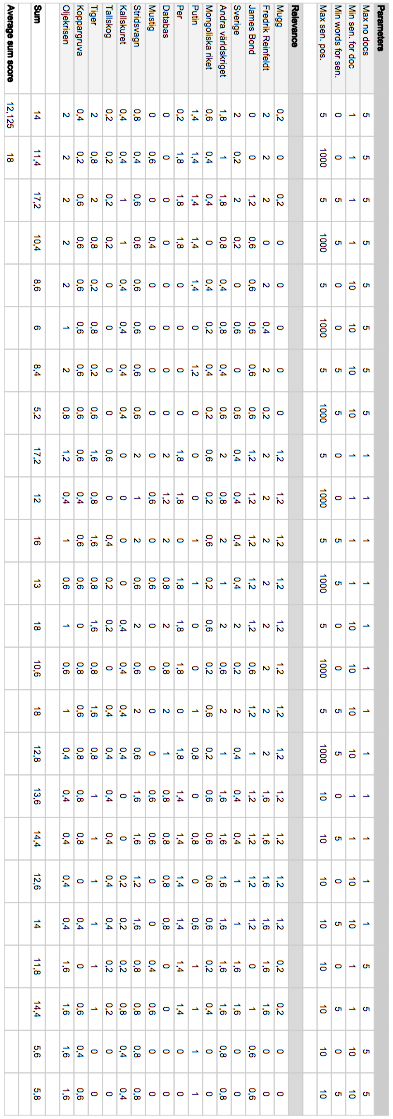
\includegraphics[width=\textwidth,height=\textheight, keepaspectratio]{data_rot.png} 
   \label{fig:data}
\end{figure}


\end{appendices}


\end{document}  